\graphicspath{{images/}{report/images/}}
\setlength{\emergencystretch}{3em}

\section{Nội dung chính của bài hướng dẫn}

Trước khi đi vào từng kỹ thuật, các công trình chính trong phần này được định vị theo vai trò mà chúng đảm nhiệm trong mạch lập luận của bài hướng dẫn.
Mỗi công trình không được trình bày như một mục tổng thuật tài liệu riêng. Thay vào đó, từng công trình được dùng để xử lý một nút thắt kỹ thuật cụ thể: học dynamics, biểu diễn chính sách, kiểm soát khai thác lỗi, tinh chỉnh diffusion model bằng reward, hoặc chuyển tương tác thành khớp phân phối.

\begin{table}[H]
\centering
\small
\setlength{\tabcolsep}{4pt}
\renewcommand{\arraystretch}{1.18}
\begin{tabular}{p{0.28\textwidth}p{0.31\textwidth}p{0.31\textwidth}}
\hline
{\raggedright\textbf{Công trình / vai trò}\par} & {\raggedright\textbf{Kỹ thuật chính}\par} & {\raggedright\textbf{Điểm cần rút ra}\par} \\
\hline
{\raggedright\textbf{PILCO, PETS, Dreamer, Diffuser}\newline Mô hình thế giới trong RL dựa trên mô hình\par} & {\raggedright Học dynamics bằng conditional likelihood hoặc model quỹ đạo\par} & {\raggedright Giảm chi phí tương tác, nhưng chịu rủi ro rollout error và model exploitation\par} \\
{\raggedright\textbf{Decision Transformer}\newline Mô hình chuỗi làm chính sách\par} & {\raggedright Conditioning chính sách trên return-to-go và history quỹ đạo\par} & {\raggedright Minh họa chính sách tạo sinh trong offline RL, nhưng dễ học correlation thay vì causal effect\par} \\
{\raggedright\textbf{Diffusion-DICE}\newline Chính sách khuếch tán trong offline RL\par} & {\raggedright Guide-then-select với density-ratio guidance và chọn candidate bằng $Q$\par} & {\raggedright Khai thác biểu diễn đa mode của diffusion mà giảm khai thác lỗi\par} \\
{\raggedright\textbf{DDPO}\newline Tinh chỉnh diffusion model bằng RL\par} & {\raggedright Xem chain khử nhiễu như finite-horizon MDP và tối ưu bằng gradient chính sách\par} & {\raggedright Cho thấy chiều ngược lại: RL có thể tối ưu chính generative model theo downstream reward\par} \\
{\raggedright\textbf{GCBC, Học tăng cường song nguyên, DICE, f-Policy Gradients}\newline Quá trình tương tác như một mô hình tạo sinh\par} & {\raggedright Goal conditioning, occupancy matching, tỉ lệ mật độ và gradient $f$-divergence\par} & {\raggedright Thay thiết kế reward bằng mục tiêu trên phân phối, nhưng vẫn phụ thuộc miền hỗ trợ và độ ổn định ước lượng\par} \\
\hline
\end{tabular}
\caption{Các công trình chính trong Phần I và Phần II được nhóm theo vai trò kỹ thuật trong mạch lập luận.}
\label{tab:tv2-method-roadmap}
\end{table}

\subsection{Mô hình tạo sinh trong hệ thống học tăng cường}

\subsubsection{So sánh mục tiêu học có giám sát và mục tiêu RL}

Điểm xuất phát của phân tích là sự khác biệt giữa học có giám sát và học tăng cường.
Trong học có giám sát, bộ dữ liệu được xem như cố định.
Nếu học một chính sách bằng imitation learning, dữ liệu gồm các cặp trạng thái--hành động $(s,a)$ từ chuyên gia hoặc từ một hệ thống có sẵn. Mô hình được tối ưu để tăng likelihood của hành động trong bộ dữ liệu:
\begin{equation}
    \max_\theta\;
    J_{\mathrm{SL}}(\theta)
    =
    \mathbb{E}_{(s,a)\sim\mathcal{D}}
    \left[
        \log \pi_\theta(a\mid s)
    \right].
    \label{eq:tv2-sl-objective}
\end{equation}
Mục tiêu này có bản chất là tái tạo hành vi quan sát được.
Trong trường hợp chính sách Gaussian với phương sai cố định, maximum likelihood tương đương với việc giảm sai số bình phương giữa hành động dự đoán và hành động trong bộ dữ liệu.
Vì vậy, chất lượng chính sách phụ thuộc trực tiếp vào chất lượng dữ liệu.
Nếu bộ dữ liệu đến từ một chính sách yếu hoặc không bao phủ những hành vi tốt, mục tiêu học có giám sát không tự tạo ra cơ chế để vượt ra khỏi giới hạn đó.

Trong RL, mô hình không chỉ học từ dữ liệu có sẵn mà còn quyết định dữ liệu nào sẽ được sinh ra.
Bài toán thường được hình thức hóa bằng một Markov Decision Process gồm state $s_t$, action $a_t$, dynamics $p(s_{t+1}\mid s_t,a_t)$, reward $r(s_t,a_t)$ và discount factor $\gamma$.
Một quỹ đạo có dạng $\tau=(s_0,a_0,s_1,a_1,\ldots)$, với return chiết khấu:
\begin{equation}
    R(\tau)
    =
    \sum_{t=0}^{\infty}
    \gamma^t r(s_t,a_t).
    \label{eq:tv2-return}
\end{equation}
Mục tiêu của RL đánh giá chính sách theo expected discounted return qua các quỹ đạo mà chính chính sách sinh ra:
\begin{equation}
    J_{\mathrm{RL}}(\theta)
    =
    \mathbb{E}_{\tau\sim\pi_\theta}
    \left[
        R(\tau)
    \right].
    \label{eq:tv2-rl-objective}
\end{equation}
Khác biệt then chốt nằm ở phân phối lấy kỳ vọng.
Trong Phương trình~\eqref{eq:tv2-sl-objective}, dữ liệu đến từ $\mathcal{D}$ và không phụ thuộc vào tham số chính sách đang học.
Trong Phương trình~\eqref{eq:tv2-rl-objective}, quỹ đạo lại được sinh bởi chính $\pi_\theta$ khi chính sách tương tác với environment.
Khi $\theta$ thay đổi, phân phối hành động thay đổi, phân phối trạng thái được ghé thăm cũng thay đổi, và do đó phân phối dữ liệu huấn luyện trong tương lai cũng thay đổi.

Do phân phối quỹ đạo phụ thuộc vào chính sách, tối ưu RL đồng thời thay đổi quy tắc ra quyết định và phân phối dữ liệu mà quy tắc đó sẽ gặp trong tương lai.
Khác với học có giám sát trên phân phối cố định, sai lệch của chính sách có thể làm thay đổi chính miền trạng thái dùng để đánh giá và cập nhật chính sách.
Đặc điểm phân phối này tạo ra mối liên hệ trực tiếp với mô hình hóa tạo sinh. Tuy nhiên, RL có thêm một ràng buộc riêng: phân phối sinh ra phải được đánh giá thông qua reward và dynamics của môi trường.

\subsubsection{Mô hình tạo sinh làm mô hình thế giới}

Vai trò trực tiếp nhất của generative models trong RL là mô hình thế giới.
Trong nhiều bài toán như robotics, điều khiển hệ thống vật lý, thiết kế phân tử hoặc tương tác với người dùng thật, thu thập dữ liệu bằng cách chạy chính sách trong môi trường có thể chậm, tốn kém hoặc nguy hiểm.
Model-based RL giải quyết khó khăn này bằng cách học một mô hình dynamics:
\begin{equation}
    p_\phi(s'\mid s,a)
    \approx
    p(s'\mid s,a).
    \label{eq:tv2-world-model}
\end{equation}
Nếu có bộ dữ liệu chuyển trạng thái $\mathcal{D}=\{(s,a,s')\}$, mô hình thế giới có thể được học bằng maximum likelihood trên các tuple $(s,a,s')$:
\begin{equation}
    \max_\phi\;
    \mathbb{E}_{(s,a,s')\sim\mathcal{D}}
    \left[
        \log p_\phi(s'\mid s,a)
    \right].
    \label{eq:tv2-world-model-mle}
\end{equation}
Về mặt huấn luyện, đây là một bài toán conditional generative modeling: từ $(s,a)$, model sinh hoặc ước lượng distribution của state kế tiếp.
Sau khi học được, mô hình thế giới có thể được dùng để rollout, đánh giá chính sách hoặc huấn luyện chính sách mà không cần tương tác trực tiếp với environment thật ở mọi bước.

Các công trình model-based RL được đặt trong phần này như các ví dụ về những generative model families có thể thay vào cùng formulation, thay vì là đối tượng khảo sát thuật toán chi tiết.
Các lựa chọn tiêu biểu gồm Gaussian process trong \textbf{PILCO}, ensemble Gaussian MLP trong \textbf{PETS}, latent state-space model trong \textbf{Dreamer}, diffusion model trên quỹ đạo trong \textbf{Diffuser}, sequence model trong \textbf{Decision Transformer} và \textbf{Trajectory Transformer}, cùng flow-matching model trong \textbf{Temporal Difference Flows}~\cite{deisenroth2011pilco,chua2018pets,hafner2019dreamer,janner2022diffuser,chen2021decision,janner2021trajectory,farebrother2025tdflows}.
Danh sách này cho thấy ``mô hình thế giới'' không chỉ định một architecture cụ thể: model family được lựa chọn quyết định cách biểu diễn uncertainty, high-dimensional observation, multimodality và độ dài của rollout, trong khi vai trò chung vẫn là xấp xỉ dynamics để hỗ trợ planning hoặc học chính sách.

\begin{figure}[H]
    \centering
    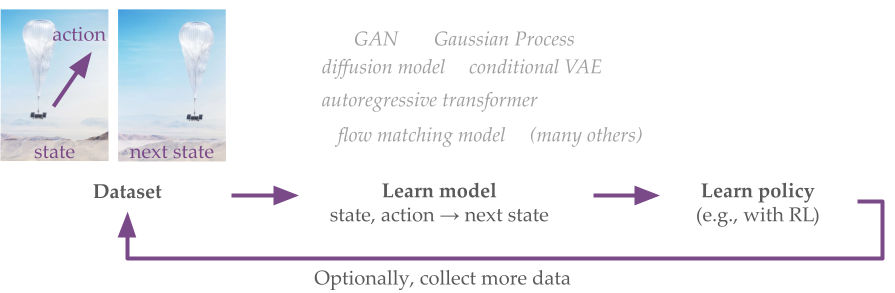
\includegraphics[width=0.95\textwidth]{notes_fig3_world_model.png}
    \caption{Pipeline model-based RL với mô hình thế giới: generative model được huấn luyện để học dynamics từ transition data, sau đó hỗ trợ học chính sách. Nguồn hình: Figure 3 trong \cite{eysenbach2025generativerl}.}
    \label{fig:tv2-notes-fig3-world-model}
\end{figure}

Mô hình thế giới đem lại lợi ích rõ ràng về chi phí tính toán: rollout trong neural model có thể chạy theo batch trên GPU, trong khi simulator thật hoặc hệ thống vật lý thật có thể rất đắt.
Lợi ích tính toán này chỉ có ý nghĩa khi sai số mô hình được kiểm soát trên rollout.
Lỗi dự đoán một bước có thể tích lũy thành sai lệch lớn sau nhiều bước, và sai lệch đó còn nguy hiểm hơn khi chính sách học cách khai thác vùng mà model dự đoán quá lạc quan về reward hoặc dynamics.
Do đó, mô hình thế giới không chỉ cần chính xác trung bình trên bộ dữ liệu ban đầu. Hệ thống còn cần cơ chế đánh giá độ tin cậy của model và quyết định khi nào phải thu thập thêm dữ liệu từ environment.
Hệ quả là độ chính xác one-step chưa đủ để đánh giá mô hình thế giới. Độ tin cậy của model còn phụ thuộc vào sai số tích lũy trên rollout và vào phân phối trạng thái do chính sách đang tối ưu tạo ra.

\subsubsection{Học có trọng số phần thưởng và hàm điểm số}

Sau mô hình thế giới, câu hỏi nền tảng là dữ liệu trong RL đến từ đâu.
Trong học có giám sát, bộ dữ liệu là đầu vào cố định và tồn tại độc lập với model đang học.
Ngược lại, trong RL, chính chính sách quyết định dữ liệu nào sẽ được thu thập. Vì vậy, cải thiện chính sách và tạo dữ liệu mới là hai quá trình phụ thuộc lẫn nhau.
Chính sách tốt cần quỹ đạo tốt để học, nhưng quỹ đạo tốt lại thường chỉ xuất hiện khi chính sách đã đủ tốt.

Quan hệ này có thể được hình thức hóa bằng một lower bound kiểu ELBO, trong đó quỹ đạo đóng vai trò latent variable.
Gọi $\pi_\theta(\tau)$ là xác suất chính sách sinh quỹ đạo $\tau$, và $R(\tau)>0$ là return.
Với một variational distribution $q(\tau)$ dương trên các quỹ đạo được xét, ta nhân và chia integrand cho $q(\tau)$:
\begin{equation}
\begin{aligned}
    \log
    \mathbb{E}_{\pi_\theta(\tau)}
    [R(\tau)]
    &=
    \log
    \int
    \pi_\theta(\tau)R(\tau)\,d\tau\\
    &=
    \log
    \int
    q(\tau)
    \frac{
        \pi_\theta(\tau)R(\tau)
    }{
        q(\tau)
    }
    d\tau.
\end{aligned}
    \label{eq:tv2-elbo-reweight}
\end{equation}
Phép biến đổi này không làm thay đổi expected return, nhưng đưa biểu thức về log của một kỳ vọng theo $q$, là dạng cần thiết để áp dụng Jensen.
Giả thiết $R(\tau)>0$ bảo đảm đối số của log dương.
Nếu return không dương, phép suy diễn này không áp dụng trực tiếp. Khi đó cần xác định một hàm trọng số dương từ return, tức là mục tiêu tái trọng số cũng thay đổi tương ứng.
Khi đó:
\begin{equation}
    \log
    \mathbb{E}_{\pi_\theta(\tau)}
    [R(\tau)]
    \geq
    \mathbb{E}_{q(\tau)}
    \left[
        \log \pi_\theta(\tau)
        +
        \log R(\tau)
        -
        \log q(\tau)
    \right].
    \label{eq:tv2-elbo}
\end{equation}
Dưới góc nhìn variational inference, quỹ đạo $\tau$ đóng vai trò như một latent variable.
Đại lượng tương ứng với evidence trong phép diễn giải này là expected return $\mathbb{E}_{\pi_\theta(\tau)}[R(\tau)]$. Phương trình~\eqref{eq:tv2-elbo} xây dựng một lower bound cho log của đại lượng đó.
Các quỹ đạo tạo ra return cao chưa được biết trước và được mô hình hóa thông qua variational distribution $q(\tau)$.

\begin{figure}[H]
    \centering
    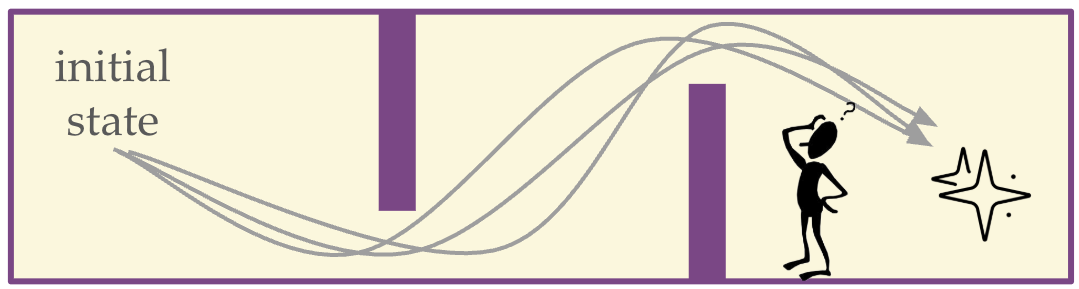
\includegraphics[width=0.74\textwidth]{notes_fig6_latent_paths.png}
    \caption{Diễn giải RL như một bài toán latent-variable. Các path dẫn đến high-reward state đóng vai trò latent variables cần được suy luận. Nguồn hình: Figure 6 trong \cite{eysenbach2025generativerl}.}
    \label{fig:tv2-notes-fig6-latent-paths}
\end{figure}

Trong một bước coordinate update, ký hiệu $\pi_{\theta_{\mathrm{old}}}$ là chính sách đã sinh batch quỹ đạo hiện tại.
Tối ưu lower bound theo $q$ với chính sách này được giữ cố định cho nghiệm:
\begin{equation}
    q^*(\tau)
    =
    \frac{
        R(\tau)\pi_{\theta_{\mathrm{old}}}(\tau)
    }{
        \int R(\tau')\pi_{\theta_{\mathrm{old}}}(\tau')d\tau'
    }.
    \label{eq:tv2-q-star-old}
\end{equation}
Phân phối $q^*$ tái trọng số quỹ đạo của chính sách cũ theo return và không tạo xác suất trên các quỹ đạo nằm ngoài support đã được lấy mẫu.
Vì vậy, policy update chỉ có thể nhấn mạnh các hành vi đã xuất hiện; khả năng khám phá vẫn quyết định những vùng quỹ đạo nào có thể được tối ưu ở bước kế tiếp.

Khi giữ $q^*$ cố định và tối ưu chính sách mới, các hằng số chuẩn hóa không phụ thuộc vào $\theta$ có thể được bỏ qua.
Sau khi giữ $q^*$ cố định, reward-weighted regression tối ưu likelihood của quỹ đạo dưới trọng số return:
\begin{equation}
    \mathcal{L}_{\mathrm{RWR}}(\theta)
    =
    \mathbb{E}_{\tau\sim\pi_{\theta_{\mathrm{old}}}}
    \left[
        R(\tau)
        \log\pi_\theta(\tau)
    \right].
    \label{eq:tv2-rwr-objective}
\end{equation}
Do likelihood quỹ đạo phân rã theo các action, gradient của mục tiêu này có dạng:
\begin{equation}
    \nabla_\theta\mathcal{L}_{\mathrm{RWR}}(\theta)
    =
    \mathbb{E}_{\tau\sim\pi_{\theta_{\mathrm{old}}}}
    \left[
        R(\tau)
        \sum_t
        \nabla_\theta
        \log\pi_\theta(a_t\mid s_t)
    \right].
    \label{eq:tv2-rwr-gradient}
\end{equation}
Kỳ vọng trong Phương trình~\eqref{eq:tv2-rwr-gradient} được lấy theo chính sách ở vòng trước, còn log-likelihood được tối ưu theo tham số chính sách mới.
Đây là cấu trúc update trong phép suy diễn ELBO của tutorial: lấy mẫu quỹ đạo, cố định batch, gán trọng số bằng return và thực hiện maximum likelihood có trọng số~\cite{peters2007rwr}.

Cần phân biệt estimator trên với gradient chính sách on-policy của expected return.
Nếu lấy gradient trực tiếp của expected return thay vì tối ưu lower bound, ta thu được estimator gradient chính sách:
\begin{equation}
    \nabla_\theta J(\theta)
    =
    \mathbb{E}_{\tau\sim\pi_\theta}
    \left[
        R(\tau)
        \sum_t
        \nabla_\theta
        \log\pi_\theta(a_t\mid s_t)
    \right].
    \label{eq:tv2-policy-gradient-on-policy}
\end{equation}
Số hạng $\nabla_\theta\log\pi_\theta(a_t\mid s_t)$ chính là hàm điểm số của chính sách.
Sự xuất hiện của cùng hàm điểm số trong Phương trình~\eqref{eq:tv2-rwr-gradient} và Phương trình~\eqref{eq:tv2-policy-gradient-on-policy} là cầu nối kỹ thuật giữa RL và generative modeling: bất kỳ generative model family nào cho phép tính hoặc ước lượng score của action đều có thể được tích hợp vào cập nhật kiểu gradient chính sách~\cite{williams1992reinforce}.
Kết quả này không phụ thuộc vào giả thiết chính sách Gaussian; transformer, diffusion model và flow model khác nhau ở cách tham số hóa phân phối và xây dựng score estimator.

\begin{figure}[H]
    \centering
    \begin{tikzpicture}[
        box/.style={draw, rounded corners=2pt, align=center, minimum width=3.2cm, minimum height=0.95cm},
        arr/.style={-{Latex[length=2mm]}, thick}
    ]
        \node[box] (gm) at (0,0) {Chính sách tạo sinh\\$\pi_\theta(a\mid s)$};
        \node[box] (score) at (4.7,0) {Hàm điểm số\\$\nabla_\theta\log\pi_\theta$};
        \node[box] (pg) at (9.5,0) {Gradient chính sách\\update};
        \node[box] (newpol) at (4.7,-2.0) {Action distribution\\được cải thiện};
        \draw[arr] (gm) -- (score);
        \draw[arr] (score) -- (pg);
        \draw[arr] (pg) -- (newpol);
        \draw[arr] (newpol.west) to[out=180,in=-70]
            node[pos=0.48, below=7pt, fill=white, inner sep=1pt]{quỹ đạo mới}
            (gm.south);
    \end{tikzpicture}
    \caption{Sơ đồ cho thấy vai trò của hàm điểm số: cùng đại lượng $\nabla_\theta\log\pi_\theta$ xuất hiện trong gradient chính sách và trong generative model, nên chính sách tạo sinh có thể được cập nhật bằng tín hiệu RL.}
    \label{fig:tv2-score-bridge-tikz}
\end{figure}

\subsubsection{Mô hình tạo sinh làm chính sách}

Khi chính sách được nhìn như phân phối có điều kiện $\pi_\theta(a\mid s)$, chính chính sách đã là một generative model sinh action từ state.
Ở mức kỹ thuật, các policy distribution đơn giản được thay bằng những kiến trúc sinh mạnh hơn, đặc biệt là sequence models và diffusion models.

Ghi chú bài giảng trước hết trừu tượng hóa hướng mô hình hóa chuỗi cho RL bằng cách xem quỹ đạo ngoại tuyến như một chuỗi trạng thái, hành động và phần thưởng~\cite{eysenbach2025generativerl}:
\begin{equation}
    S_t,\; A_t,\; R_{t+1},\; S_{t+1},\; A_{t+1},\ldots
    \label{eq:tv2-sequence-trajectory}
\end{equation}
Trong công trình \textbf{Decision Transformer}, ý tưởng này được cụ thể hóa bằng một autoregressive transformer không học hàm giá trị hoặc Bellman backup trực tiếp, mà học phân phối hành động có điều kiện trên return-to-go và lịch sử quỹ đạo~\cite{chen2021decision}:
$\pi(a_t\mid s_{\leq t},a_{<t},R_{\mathrm{target}})$, thay cho conditioning chỉ trên state hiện tại.
Giá trị return mục tiêu đóng vai trò biến điều kiện điều chỉnh phân phối hành động học được từ dữ liệu offline.
Điểm mạnh của cách tiếp cận này là tận dụng năng lực sequence modeling đã thành công trong generative AI.
Hạn chế là mô hình chủ yếu học correlation trong offline quỹ đạo.
Nếu một quỹ đạo có return cao do may mắn trong môi trường stochastic, việc condition trên return cao có thể khiến mô hình bắt chước action không thực sự là nguyên nhân tạo ra reward cao~\cite{paster2022luck}.
Vì vậy, vai trò của \textbf{Decision Transformer} trong phần này không phải là thay thế toàn bộ RL bằng language modeling, mà là minh họa một policy class mới: chính sách được mô hình hóa như conditional sequence model.
Nút thắt kỹ thuật mà công trình này làm rõ là sự khác biệt giữa biểu diễn một phân phối hành động phức tạp và bảo đảm policy improvement khi dữ liệu chỉ đến từ offline quỹ đạo.

Diffusion chính sách mở rộng ý tưởng chính sách tạo sinh sang phân phối hành động đa mode.
Trong offline RL, cùng một state có thể có nhiều action hợp lệ do bộ dữ liệu chứa nhiều chiến lược khác nhau.
Một Gaussian chính sách đơn mode có thể trung bình hóa các mode và sinh action không thuộc mode nào.
Ngược lại, diffusion model có thể sinh action qua nhiều bước khử nhiễu và biểu diễn phân phối phức tạp hơn.
Tuy nhiên, expressivity cao không tự bảo đảm policy improvement: khi diffusion chính sách được kết hợp với critic trong offline RL, các candidate ngoài support dữ liệu có thể nhận giá trị dự đoán sai.
\textbf{Diffusion-DICE} tập trung vào chính tương tác giữa khả năng sinh đa mode và sai số ngoại suy của critic.

\subsubsection{Nghiên cứu trường hợp: Diffusion-DICE}

\textbf{Diffusion-DICE} là case study trung tâm cho diffusion chính sách trong offline RL~\cite{mao2024diffusiondice}.
Vấn đề kỹ thuật của phương pháp là tận dụng khả năng sinh action đa mode của diffusion model mà không để critic kéo chính sách ra khỏi support của dữ liệu.
Trong diffusion chính sách, action sạch $a_0$ được sinh từ chuỗi khử nhiễu $a_T,\ldots,a_0$ có điều kiện trên state $s$.
Mục tiêu không chỉ là bắt chước behavior chính sách trong bộ dữ liệu, mà là sinh action có giá trị cao theo reward hoặc hàm Q.
Nút thắt mà công trình này xử lý là một điểm yếu cụ thể của diffusion chính sách trong offline RL: model đủ mạnh để sinh nhiều candidate actions, nhưng critic học từ dữ liệu offline có thể đánh giá sai các candidate nằm ngoài support.
Do đó, kỹ thuật cốt lõi không chỉ là thêm guidance vào diffusion sampling, mà là kiểm soát cách guidance được dùng để tránh khai thác lỗi.

Hai hướng tiếp cận chính là guide-based và select-based.
Guide-based methods học diffusion behavior chính sách rồi thêm guidance term để đẩy quá trình sampling về vùng có giá trị cao:
\begin{equation}
    \nabla_{a_t}
    \log \pi_t(a_t\mid s)
    =
    \nabla_{a_t}
    \log \pi_t^D(a_t\mid s)
    +
    \nabla_{a_t}J_t(a_t,s).
    \label{eq:tv2-guide-score}
\end{equation}
Ở đây $\pi_t^D$ là behavior diffusion chính sách, còn $J_t$ là tín hiệu hướng dẫn học từ critic hoặc mục tiêu liên quan đến reward.
Đối với nhóm select-only, một cách triển khai điển hình là sinh nhiều candidate actions từ behavior chính sách rồi tái lấy mẫu theo trọng số do critic cung cấp:
\begin{equation}
    \Pr[a=a_0^j\mid s]
    =
    \frac{
        w(s,a_0^j)
    }{
        \sum_{i=1}^{N} w(s,a_0^i)
    }.
    \label{eq:tv2-select-policy}
\end{equation}
Phương trình~\eqref{eq:tv2-select-policy} mô tả cơ chế resampling của nhóm baseline select-based, chẳng hạn \textbf{IDQL}; đây chưa phải bước Select cuối cùng của Diffusion-DICE~\cite{hansenestruch2023idql}.
Cả hai hướng đều phụ thuộc vào critic.
Trong offline RL, critic chỉ được học từ bộ dữ liệu cố định; vì vậy critic có thể overestimate các action ngoài phân phối.
Nếu sampling hoặc guidance đưa action ra khỏi vùng dữ liệu, chính sách có thể khai thác lỗi critic thay vì tìm action thật sự tốt.
Hiện tượng này được gọi là khai thác lỗi.

Diffusion-DICE đề xuất paradigm guide-then-select.
Bước guide dùng score của behavior chính sách cộng với guidance liên quan đến optimal distribution ratio để sinh candidate actions.
Điểm cần trình bày cẩn thận là guidance term này không được tính bằng một closed-form đơn giản trong thực tế.
Theo Diffusion-DICE, thành phần liên quan đến tỉ lệ mật độ thường intractable vì đòi hỏi các kỳ vọng điều kiện; phương pháp biến đổi bài toán thành mục tiêu có thể học in-sample.
Sau đó, Diffusion-DICE thực hiện lựa chọn cứng trong tập $K$ candidate actions được sinh từ optimal policy distribution $\pi^*(a\mid s)$ mà bước Guide xấp xỉ.
Đặt $\mathcal{C}_K(s)=\{a_0^1,\ldots,a_0^K\}$ với $a_0^k\sim\pi^*(\cdot\mid s)$, bước Select được viết:
\begin{equation}
    \pi(s)
    =
    a^*
    \triangleq
    \underset{a\in\mathcal{C}_K(s)}{\arg\max}
    \;Q^*(s,a).
    \label{eq:tv2-diffusion-dice-select}
\end{equation}
Khác với phép resampling trong Phương trình~\eqref{eq:tv2-select-policy}, Phương trình~\eqref{eq:tv2-diffusion-dice-select} chọn candidate có giá trị $Q$ lớn nhất, thay vì gán xác suất lựa chọn tỉ lệ với trọng số~\cite{mao2024diffusiondice}.
Nhờ vậy, critic vẫn được dùng để chọn action tốt hơn, nhưng quá trình lựa chọn được giữ gần vùng dữ liệu hơn.

\begin{figure}[H]
    \centering
    \resizebox{\textwidth}{!}{%
    \begin{tikzpicture}[
        box/.style={draw, rounded corners=2pt, align=center, minimum width=2.9cm, minimum height=0.95cm},
        arr/.style={-{Latex[length=2mm]}, thick}
    ]
        \node[box] (data) at (0,0) {Offline data\\$d^D(s,a)$};
        \node[box] (guide) at (3.9,0) {Guide\\behavior score\\+ density-ratio signal};
        \node[box] (cand) at (7.8,0) {Candidate\\actions};
        \node[box] (select) at (11.7,0) {Select\\with $Q$};
        \node[box] (act) at (15.2,0) {Final\\action};
        \draw[arr] (data) -- (guide);
        \draw[arr] (guide) -- (cand);
        \draw[arr] (cand) -- (select);
        \draw[arr] (select) -- (act);
    \end{tikzpicture}
    }
    \caption{Luồng guide-then-select trong Diffusion-DICE: Guide tạo candidate actions bằng behavior score và density-ratio signal, còn Select chỉ dùng hàm Q sau khi candidate đã được giữ gần support dữ liệu.}
    \label{fig:tv2-diffusion-dice-tikz}
\end{figure}

Toycase 2D bandit cô lập chính xác vấn đề này.
Bộ dữ liệu offline chỉ bao phủ một vùng hình khuyên (annular region).
True reward cao ở outer circle, nhưng learned critic lại overestimate một số vùng inner circle do thiếu dữ liệu.
Guide-only có thể bị kéo mạnh vào vùng critic overestimate, còn select-only bị giới hạn bởi chất lượng candidate.
Diffusion-DICE giảm rủi ro bằng cách kết hợp hai bước: guide để tạo candidate hướng tới phân phối tối ưu, và select để chọn trong tập candidate theo hướng in-sample.
\textbf{QGPO} và \textbf{IDQL} có thể được xem như các baseline đại diện cho hai cực guide-only và select-only, nhưng trọng tâm kỹ thuật của phần này là cơ chế guide-then-select của Diffusion-DICE~\cite{lu2023qgpo,hansenestruch2023idql}.

\begin{figure}[H]
    \centering
    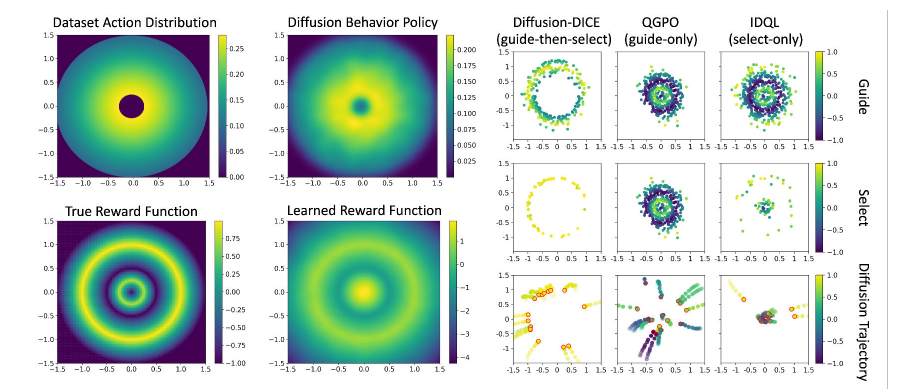
\includegraphics[width=\textwidth]{notes_fig7_diffusion_dice_full.png}
    \caption{Toycase 2D bandit của Diffusion-DICE: action trong bộ dữ liệu nằm trong vùng hình khuyên; true reward cao ở outer circle; learned reward overestimate inner circle; Diffusion-DICE giảm khai thác lỗi tốt hơn các hướng guide-only hoặc select-only. Nguồn hình: Figure 7 trong \cite{eysenbach2025generativerl}.}
    \label{fig:tv2-notes-fig7-diffusion-dice}
\end{figure}

\subsubsection{DDPO: xem quá trình khử nhiễu như một MDP}

Nếu Diffusion-DICE dùng diffusion model để xây chính sách cho RL, \textbf{DDPO} đi theo chiều ngược lại: dùng RL để fine-tune diffusion model theo downstream reward~\cite{black2024ddpo}.
Động lực của DDPO là nhiều mục tiêu quan trọng trong image generative models không được mô tả tốt bằng maximum likelihood.
Aesthetic quality, prompt-image alignment hoặc compressibility là các tiêu chí được đánh giá ở mẫu cuối, không phải likelihood của từng bước huấn luyện diffusion.
Do đó, fine-tuning bằng reward trở thành một bài toán RL tự nhiên.
Ba thành phần kỹ thuật xác định \textbf{DDPO}: reward chỉ xuất hiện ở mẫu cuối, chuỗi khử nhiễu cung cấp một dãy decision steps, và gradient chính sách phân bổ tín hiệu reward cuối về từng transition khử nhiễu.
Nhờ đó, DDPO trở thành một formulation RL đầy đủ cho quá trình sampling của diffusion model, thay vì chỉ là một thủ thuật tái trọng số các mẫu cuối có reward cao.

Trong diffusion sampling, một mẫu cuối $x_0$ được tạo ra từ chuỗi khử nhiễu:
\begin{equation}
    x_T \rightarrow x_{T-1} \rightarrow \cdots \rightarrow x_0.
    \label{eq:tv2-denoising-chain}
\end{equation}
DDPO mô hình hóa chuỗi này như một finite-horizon MDP.
Với prompt hoặc context $c$, state tại timestep $t$ là noisy sample $x_t$.
Action không nên hiểu cứng là predicted noise; cách mô tả đúng hơn là quyết định khử nhiễu, tức lấy mẫu $x_{t-1}$ từ chính sách:
\begin{equation}
    p_\theta(x_{t-1}\mid x_t,c).
    \label{eq:tv2-ddpo-policy}
\end{equation}
Reward được chấm ở mẫu cuối, ký hiệu chung là $r(x_0,c)$; các ví dụ được DDPO khảo sát gồm compressibility, aesthetic quality và prompt--image alignment~\cite{black2024ddpo}.
Theo bài báo DDPO, khi đó mục tiêu là kỳ vọng reward trên quỹ đạo khử nhiễu, và policy-gradient estimator có dạng:
\begin{equation}
    \nabla_\theta J(\theta)
    =
    \mathbb{E}
    \left[
        r(x_0,c)
        \sum_{t=1}^{T}
        \nabla_\theta
        \log p_\theta(x_{t-1}\mid x_t,c)
    \right].
    \label{eq:tv2-ddpo-gradient}
\end{equation}
Công thức này cho thấy reward cuối được gán credit cho toàn bộ chuỗi transition khử nhiễu.
So với reward-weighted regression, DDPO giữ lại cấu trúc nhiều bước của quá trình sampling.
RWR chỉ tăng likelihood của mẫu cuối có reward cao, trong khi DDPO cập nhật log-probability của từng transition $x_t\rightarrow x_{t-1}$.
Theo bài báo DDPO, cách tiếp cận này hiệu quả hơn RWR trong các mục tiêu được khảo sát vì RWR gặp các vấn đề optimization và approximation trong diffusion setting~\cite{black2024ddpo}.

Ở mức cụ thể hóa trong bài báo gốc, formulation này dẫn tới hai estimator.
\textbf{DDPO-SF} áp dụng trực tiếp score-function estimator theo tinh thần REINFORCE trên các quỹ đạo khử nhiễu.
\textbf{DDPO-IS} bổ sung importance sampling để tái sử dụng quỹ đạo đã thu thập cho nhiều bước cập nhật hơn, đồng thời dùng clipping theo tinh thần PPO nhằm kiểm soát policy shift.
Các chi tiết này thuộc phần triển khai của bài báo DDPO; trong tutorial, vai trò chính của DDPO là minh họa việc xem khử nhiễu như MDP và tối ưu diffusion model bằng gradient chính sách~\cite{black2024ddpo}.

Trong formulation tổng quát của DDPO, chuỗi khử nhiễu được xem như một MDP và được tối ưu bằng gradient chính sách thay cho reward-weighted likelihood.
Bài báo gốc cho thấy formulation này có thể fine-tune image generative models theo các downstream criteria như aesthetics, compressibility và prompt--image alignment hiệu quả hơn RWR trong các thiết lập được khảo sát; tuy nhiên, tối ưu một reward proxy không hoàn chỉnh vẫn có thể dẫn tới overoptimization hoặc reward hacking~\cite{black2024ddpo,black2024ddpoproject}.

Trong mạch lập luận chung, DDPO hoàn thiện quan hệ hai chiều giữa hai lĩnh vực.
Diffusion-DICE đưa diffusion model vào RL để biểu diễn chính sách phức tạp. Ngược lại, DDPO đưa policy optimization vào diffusion model để điều chỉnh chính quá trình sampling.
Cả hai công trình đều sử dụng cấu trúc nhiều bước của diffusion, nhưng tối ưu hai đối tượng khác nhau. Diffusion-DICE tìm action có giá trị cao trong offline RL. DDPO tối ưu chất lượng mẫu cuối theo downstream reward.

\subsection{Quá trình tương tác như một mô hình tạo sinh}

\subsubsection{Cách chính sách và environment sinh dữ liệu}

Góc nhìn thứ hai xem toàn bộ quá trình tương tác giữa chính sách và environment như một generative model.
Một diffusion model tạo ảnh bằng nhiều bước khử nhiễu.
Tương tự, một RL agent tạo observation tương lai bằng nhiều bước tương tác. Chính sách sinh action, environment sinh state kế tiếp, rồi quá trình lặp lại.
Nếu $s_0$ là trạng thái ban đầu, quá trình
\begin{equation}
    a_t\sim\pi(a_t\mid s_t),
    \qquad
    s_{t+1}\sim p(s_{t+1}\mid s_t,a_t)
    \label{eq:tv2-interaction-dynamics}
\end{equation}
xác định một phân phối trên các state hoặc observation tương lai.
Trong cách nhìn này, hệ agent--environment là một quá trình tạo sinh. Mẫu sinh ra không phải là ảnh, mà là trạng thái hoặc observation mà agent đạt được sau nhiều bước tương tác.

Ba động lực kỹ thuật làm cho cách mô hình hóa này hữu ích trong bối cảnh GenAI và RL.
Động lực thứ nhất là RL cung cấp ngôn ngữ hình thức để mô tả hệ thống sinh có tương tác với con người, công cụ hoặc môi trường vật lý, kể cả khi một phần quá trình là hộp đen hoặc không khả vi.
Động lực thứ hai là đặc tả tác vụ bằng scalar reward thường đòi hỏi reward engineering và reward shaping thủ công. Các thành phần trung gian có thể vô tình mã hóa trước cách giải thay vì chỉ mô tả kết quả mong muốn.
Động lực thứ ba là scalar reward tạo ra sự lệch pha với mô hình hóa tạo sinh thông thường, nơi supervision được cung cấp dưới dạng dữ liệu mẫu.
Part II khảo sát khả năng đặc tả một lớp bài toán RL bằng desired observations hoặc goal data. Cách này chuyển một phần bài toán từ reward engineering sang khớp phân phối trên outcome~\cite{eysenbach2025generativerl}.

\begin{figure}[H]
    \centering
    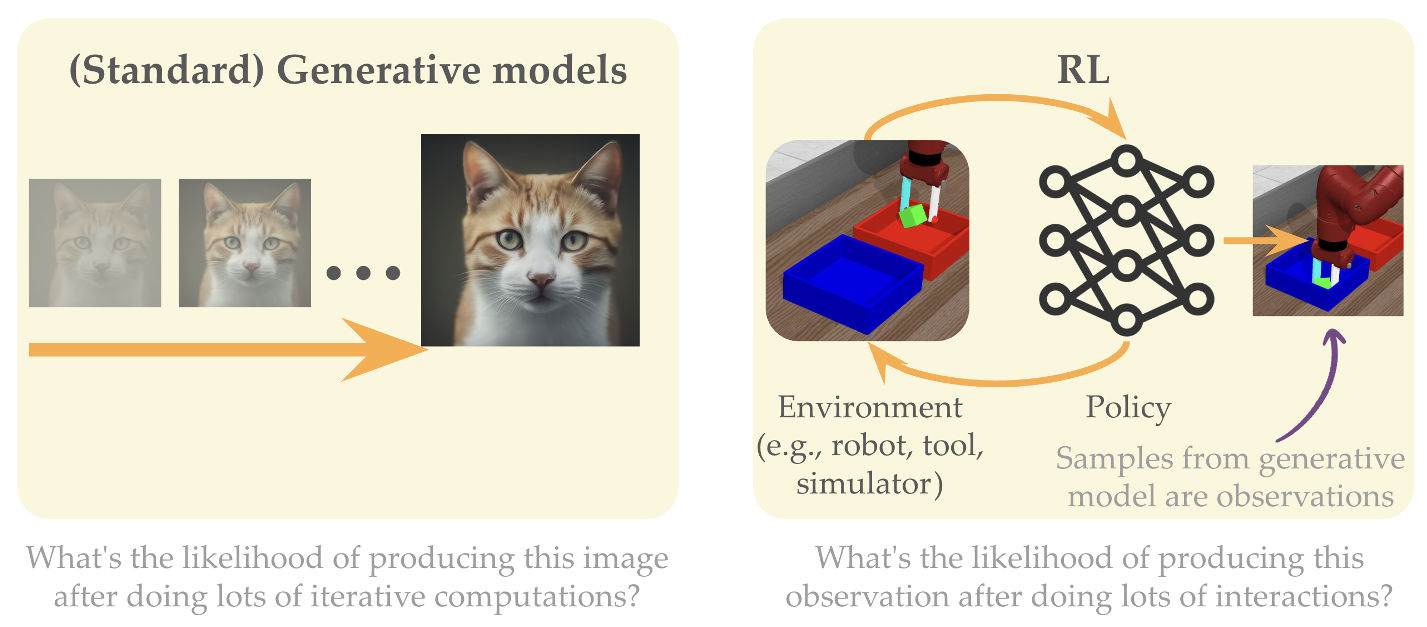
\includegraphics[width=0.88\textwidth]{notes_fig8_interaction_generative_model.png}
    \caption{So sánh generative models chuẩn với tương tác trong RL. Cả hai đều dùng nhiều bước tính toán hoặc tương tác để tạo mẫu. Nguồn hình: Figure 8 trong \cite{eysenbach2025generativerl}.}
    \label{fig:tv2-notes-fig8-interaction}
\end{figure}

Cách nhìn này không yêu cầu toàn bộ chuỗi sinh phải được biểu diễn bởi một mạng khả vi: chính sách, environment, tool và human feedback chỉ cần cùng xác định một distribution trên outcome.
Bài toán điều khiển sau đó có thể được phát biểu dưới dạng thay đổi chính sách để tăng likelihood của các outcome mong muốn, với đạt đích là trường hợp cụ thể được phân tích tiếp theo.

\begin{figure}[H]
    \centering
    \resizebox{0.92\textwidth}{!}{%
    \begin{tikzpicture}[
        box/.style={draw, rounded corners=2pt, align=center, minimum width=2.35cm, minimum height=0.85cm},
        arr/.style={-{Latex[length=2mm]}, thick}
    ]
        \node[box] (s0) at (0,0) {$s_0$};
        \node[box] (pi0) at (2.8,0) {chính sách\\$\pi(a_0\mid s_0)$};
        \node[box] (env0) at (5.9,0) {environment\\$p(s_1\mid s_0,a_0)$};
        \node[box] (s1) at (9.1,0) {$s_1$};
        \node[box] (pi1) at (9.1,-2.0) {chính sách\\$\pi(a_1\mid s_1)$};
        \node[box] (env1) at (12.2,-2.0) {environment\\$p(s_2\mid s_1,a_1)$};
        \node[box] (sf) at (15.3,-2.0) {mẫu tương lai\\$s_f$};
        \draw[arr] (s0) -- (pi0);
        \draw[arr] (pi0) -- (env0);
        \draw[arr] (env0) -- (s1);
        \draw[arr] (s1) -- (pi1);
        \draw[arr] (pi1) -- (env1);
        \draw[arr] (env1) -- (sf);
    \end{tikzpicture}
    }
    \caption{Quá trình tương tác tạo sinh: mỗi bước chính sách sinh action, environment sinh state kế tiếp, và toàn bộ vòng lặp tạo ra mẫu tương lai $s_f$.}
    \label{fig:tv2-interaction-tikz}
\end{figure}

\subsubsection{Đạt đích và thước đo chiếm dụng}

Đạt đích là thiết lập đơn giản nhất cho quan điểm xem quá trình tương tác như một mô hình tạo sinh.
Thay vì reward engineering thủ công nhiều thành phần, task được mô tả bằng một observation mong muốn $g$.
Đạt đích trước hết có thể được hiểu bằng trực giác indicator trong finite-state setting: agent nhận tín hiệu dương khi đạt goal và nhận tín hiệu bằng không ở các trạng thái khác.
Để có formulation áp dụng được cho cả observation rời rạc lẫn liên tục, mục tiêu chính được viết qua xác suất transition tới goal:
\begin{equation}
    \max_\pi
    (1-\gamma)
    \mathbb{E}_{\pi}
    \left[
        \sum_{t=0}^{\infty}
        \gamma^t
        p(s_{t+1}=g\mid s_t,a_t)
    \right].
    \label{eq:tv2-goal-prob}
\end{equation}
Hệ số $(1-\gamma)$ chuẩn hóa tổng chiết khấu thành một phân phối.
Mục tiêu này tương đương một bài toán RL chuẩn với reward được định nghĩa từ xác suất đạt observation mong muốn:
\begin{equation}
    r_g(s,a)
    =
    (1-\gamma)
    p(s'=g\mid s,a).
    \label{eq:tv2-goal-reward}
\end{equation}
Reward ở đây không phải reward thủ công theo nhiều rule, mà được định nghĩa từ xác suất đạt observation mong muốn.
Điều này chuyển reward engineering sang bài toán likelihood của outcome.

Discounted state thước đo chiếm dụng mô tả phân phối state tương lai do chính sách sinh ra:
\begin{equation}
    p^\pi(s_f)
    \triangleq
    (1-\gamma)
    \mathbb{E}_{\pi}
    \left[
        \sum_{t=0}^{\infty}
        \gamma^t
        p(s_{t+1}=s_f\mid s_t,a_t)
    \right].
    \label{eq:tv2-state-occupancy}
\end{equation}
Nếu quá trình tương tác là một generative model, $p^\pi(s_f)$ chính là phân phối mẫu mà model tạo ra.
Đạt đích khi đó trở thành bài toán điều chỉnh chính sách sao cho phân phối $p^\pi$ đặt xác suất cao lên goal hoặc goal distribution.

\begin{figure}[H]
    \centering
    \resizebox{0.92\textwidth}{!}{%
    \begin{tikzpicture}[
        box/.style={draw, rounded corners=2pt, align=center, minimum width=3.6cm, minimum height=1.0cm},
        smallbox/.style={draw, rounded corners=2pt, align=center, minimum width=2.45cm, minimum height=0.85cm},
        arr/.style={-{Latex[length=2mm]}, thick}
    ]
        \node[box] (manual) at (0,0) {Manual reward\\engineering};
        \node[smallbox] (term1) at (4.2,1.1) {distance\\terms};
        \node[smallbox] (term2) at (4.2,0) {constraint\\penalties};
        \node[smallbox] (term3) at (4.2,-1.1) {task-specific\\rules};
        \node[box] (goal) at (8.8,0) {Đạt đích\\desired observation $g$};
        \node[box] (occ) at (13.3,0) {Increase\\$p^\pi(s_f=g)$};
        \draw[arr] (manual) -- (term1);
        \draw[arr] (manual) -- (term2);
        \draw[arr] (manual) -- (term3);
        \draw[arr] (term1) -- (goal);
        \draw[arr] (term2) -- (goal);
        \draw[arr] (term3) -- (goal);
        \draw[arr] (goal) -- (occ);
    \end{tikzpicture}
    }
    \caption{Đạt đích thay nhiều thành phần reward thủ công bằng một desired observation $g$; mục tiêu kỹ thuật là tăng xác suất $p^\pi(s_f=g)$.}
    \label{fig:tv2-goal-reaching-tikz}
\end{figure}

Hạn chế của đạt đích là không phải mọi tác vụ đều có thể được đặc tả bằng một trạng thái đích đơn lẻ.
Chẳng hạn, trạng thái ``căn phòng sạch'' có thể tương ứng với nhiều cấu hình quan sát hợp lệ, trong khi tiêu chí ``chuyến bay êm'' phụ thuộc vào các ràng buộc được duy trì trên toàn quỹ đạo.
Về mặt kỹ thuật, các ví dụ này đại diện cho tác vụ có nhiều outcome tương đương hoặc có constraints trên quỹ đạo, do đó không thể quy về một goal observation duy nhất.
Do đó, đạt đích chỉ là một trường hợp đặc biệt của bài toán điều khiển phân phối outcome; các tác vụ tổng quát hơn đòi hỏi formulation trên distribution quỹ đạo hoặc reward function đầy đủ.

\subsubsection{Goal-conditioned sao chép hành vi}

\textbf{Goal-Conditioned Behavioral Cloning (GCBC)} khai thác cấu trúc quỹ đạo để học chính sách hướng goal từ dữ liệu.
Trong nhóm công trình về tương tác như một mô hình tạo sinh, GCBC đóng vai trò baseline theo kiểu học có giám sát.
Nó tận dụng quỹ đạo có sẵn bằng cách dùng observation tương lai làm goal label.
Sau đó, Học tăng cường song nguyên và DICE mở rộng ý tưởng này lên mức occupancy-level khớp phân phối.
Từ một quỹ đạo trong bộ dữ liệu, ta chọn một future state $s_f$ làm goal, rồi huấn luyện chính sách sinh action hiện tại có điều kiện trên goal:
\begin{equation}
    \max_\theta
    \mathbb{E}_{\tau\sim\mathcal{D}}
    \left[
        \mathbb{E}_{(s,a,s_f)\sim\tau}
        \left[
            \log \pi_\theta(a\mid s,g=s_f)
        \right]
    \right].
    \label{eq:tv2-gcbc}
\end{equation}
\paragraph{Diễn giải Bayes.}
Phương trình~\eqref{eq:tv2-gcbc} có hình thức của sao chép hành vi với biến điều kiện goal, nhưng Bayes rule cho thấy mục tiêu còn mã hóa xác suất đạt future state.
Action được ưu tiên không chỉ vì nó xuất hiện trong dữ liệu, mà vì trong quỹ đạo gốc nó nằm trên đường dẫn đến future state được chọn làm goal.
Một cách viết bỏ qua các hằng số không phụ thuộc action là:
\begin{equation}
    \mathbb{E}_{a\sim\pi_\theta(a\mid s,g)}
    \left[
        \log p(s_f=g\mid s,a)
        +
        \log \beta(a\mid s)
    \right],
    \label{eq:tv2-gcbc-bayes}
\end{equation}
trong đó $\beta(a\mid s)$ là behavior chính sách, còn $p(s_f=g\mid s,a)$ là xác suất đạt future goal khi bắt đầu từ $(s,a)$ và tiếp tục theo chính sách đang xét.
Hạng tử đầu khuyến khích action làm tăng khả năng đạt goal.
Hạng tử thứ hai regularize action về vùng hành vi trong bộ dữ liệu.
GCBC do đó kết hợp tín hiệu đạt đích với regularization về behavior support, thay vì chỉ sao chép marginal action distribution.

\paragraph{Diễn giải bằng mặt nạ (masking).}
Diễn giải trọng tâm thứ hai xem GCBC như một bài toán masked sequence modeling trên quỹ đạo.
Trong language modeling, masking che một phần token rồi học dự đoán token bị che.
Trong modeling quỹ đạo, có thể che action hoặc state rồi yêu cầu mô hình khôi phục phần thiếu.
Với GCBC, state hiện tại và goal tương lai đóng vai trò context, còn action là phần cần dự đoán.
Nếu mask action, mô hình hoạt động như chính sách. Nếu mask future state, cùng kiến trúc hoạt động như mô hình thế giới.
Sự thay đổi vai trò được quyết định bởi biến nào được quan sát và biến nào phải sinh, chứ không nhất thiết bởi một kiến trúc riêng cho từng chức năng.

GCBC cho thấy một cách tận dụng offline quỹ đạo bằng học có giám sát. Tuy nhiên, chính sách học được vẫn bị ràng buộc mạnh bởi behavior support và các future states đã xuất hiện trong dữ liệu.
Để phân tích các phương pháp vượt ra ngoài việc clone trực tiếp hành vi, cần chuyển từ likelihood của action sang phân phối occupancy mà chính sách tạo ra.
Ở mức on-policy, f-divergence gradient cung cấp một cầu nối tự nhiên giữa khớp phân phối goal và gradient chính sách. Trong offline setting, yêu cầu học từ bộ dữ liệu cố định dẫn tới các formulation dual và DICE được trình bày tiếp theo~\cite{eysenbach2025generativerl}.

\subsubsection{Học tăng cường song nguyên và DICE}

Đạt đích yêu cầu ước lượng xác suất đạt goal, nhưng density estimation trực tiếp trong không gian observation cao chiều thường khó.
\textbf{Học tăng cường song nguyên} giải quyết vấn đề này bằng cách làm việc với thước đo chiếm dụng và khớp phân phối.
Thay vì tối ưu trực tiếp trên chính sách, ta xét state-action occupancy $d^\pi(s,a)$ do chính sách tạo ra.
Một mục tiêu có regularization có dạng:
\begin{equation}
    \max_\pi
    \;
    \mathbb{E}_{(s,a)\sim d^\pi}
    [r(s,a)]
    -
    \alpha
    D_f(d^\pi(s,a)\Vert d^O(s,a)),
    \label{eq:tv2-regularized-occupancy}
\end{equation}
trong đó $d^O$ là phân phối tham chiếu và $D_f$ là $f$-divergence.
Occupancy distribution không thể tùy ý. Nó phải thỏa các Bellman-flow constraints do dynamics quy định.
Một dạng ràng buộc Bellman-flow tương ứng với primal-Q trong notes là:
\begin{equation}
    d(s,a)
    =
    (1-\gamma)d_0(s)\pi(a\mid s)
    +
    \gamma
    \sum_{s',a'}
    d(s',a')p(s\mid s',a')\pi(a\mid s),
    \quad \forall s,a.
    \label{eq:tv2-bellman-flow}
\end{equation}
Ràng buộc này đảm bảo $d(s,a)$ là một thước đo chiếm dụng hợp lệ, tức nó có thể được sinh ra bởi một chính sách trong MDP thay vì là một phân phối tùy ý trên state-action pairs.
Bằng Lagrangian duality và convex conjugate, các ràng buộc flow có thể được chuyển thành mục tiêu theo các biến dual như $Q(s,a)$ hoặc $V(s)$.
Ví dụ, một dạng dual-V được notes trình bày là:
\begin{equation}
\begin{aligned}
    \min_V\quad
    &(1-\gamma)\mathbb{E}_{s\sim d_0}[V(s)]
    +
    \alpha
    \mathbb{E}_{(s,a)\sim d^O}
    \left[
        f_p^*
        \left(
            \frac{\mathcal{T}V(s,a)-V(s)}{\alpha}
        \right)
    \right],
\end{aligned}
    \label{eq:tv2-dual-v}
\end{equation}
trong đó $\mathcal{T}V(s,a)$ là Bellman target của $V$ và $f_p^*$ là biến thể convex conjugate dùng để xử lý ràng buộc không âm của occupancy.
Ý nghĩa kỹ thuật là bài toán khớp phân phối có thể được học bằng loss trên dữ liệu logged, thay vì yêu cầu tương tác on-policy liên tục.

\textbf{DICE methods} là họ phương pháp tiêu biểu cho ý tưởng này.
Trong offline setting, DICE xét mục tiêu:
\begin{equation}
    \pi^*
    =
    \arg\max_\pi
    \mathbb{E}_{(s,a)\sim d^\pi}
    [r(s,a)]
    -
    \alpha
    D_f(d^\pi\Vert d^D),
    \label{eq:tv2-dice-objective}
\end{equation}
trong đó $d^D$ là distribution của dữ liệu offline, tức phân phối state-action pairs đã được ghi nhận trước khi học chính sách mới.
Bài toán trực tiếp khó vì $d^\pi$ phụ thuộc vào chính sách và dynamics.
Sau biến đổi dual, mục tiêu có thể được ước lượng từ các mẫu $(s,a,s')$ trong dataset.
Tính in-sample của DICE nằm ở việc các loss dual được đánh giá trên transition đã ghi nhận, qua đó tránh yêu cầu truy vấn giá trị của toàn bộ không gian action ngoài support dữ liệu.
Trong triển khai thực tế, notes trình bày một dạng semi-gradient dùng $Q(s,a)$ để xấp xỉ Bellman target và $V(s)$ để biểu diễn biến dual theo state:
\begin{equation}
\begin{aligned}
    \min_V\quad
    &
    \mathbb{E}_{(s,a)\sim d^D}
    \left[
        (1-\gamma)V(s)
        +
        \alpha f^*
        \left(
            \frac{Q(s,a)-V(s)}{\alpha}
        \right)
    \right],\\
    \min_Q\quad
    &
    \mathbb{E}_{(s,a,s')\sim d^D}
    \left[
        r(s,a)
        +
        \gamma V(s')
        -
        Q(s,a)
    \right]^2 .
\end{aligned}
    \label{eq:tv2-dice-semi-gradient}
\end{equation}
Hai loss này chỉ cần các transition đã ghi trong dữ liệu offline, nên phù hợp với mục tiêu in-sample của DICE methods.

Một đại lượng trung tâm là stationary distribution ratio:
\begin{equation}
    w^*(s,a)
    :=
    \frac{d^*(s,a)}{d^D(s,a)}.
    \label{eq:tv2-density-ratio}
\end{equation}
Tỉ số này cho biết state-action pair trong bộ dữ liệu nên được nhấn mạnh hơn hay ít hơn để tiến đến occupancy tối ưu.
Từ góc nhìn tổng hợp của nhóm, tỉ lệ mật độ ở đây cũng cung cấp một cách diễn giải cho guidance trong Diffusion-DICE: cả hai đều mô tả sự dịch chuyển từ behavior distribution về phía optimal distribution, trong khi ràng buộc in-sample hạn chế khai thác lỗi.
Liên hệ này là phép đối chiếu giữa hai phần của tutorial, không phải một đồng nhất thức được lecture notes phát biểu trực tiếp~\cite{eysenbach2025generativerl,mao2024diffusiondice}.

\subsubsection{\texorpdfstring{$f$-Policy Gradients}{f-Policy Gradients} và state-MaxEnt RL}

Dual formulation cho biết cách biểu diễn bài toán bằng thước đo chiếm dụng và tỉ lệ mật độ.
Từ formulation này, câu hỏi trực tiếp hơn là: nếu goal được mô tả bởi một phân phối trạng thái đích $p_g(s)$, chính sách cần được cập nhật như thế nào để phân phối trạng thái mà agent tạo ra tiến gần tới phân phối này?
Gọi $p_\theta(s)$ là discounted state distribution sinh bởi chính sách $\pi_\theta$.
Bài toán khớp phân phối được viết dưới dạng:
\begin{equation}
    J(\theta)
    =
    D_f\!\left(
        p_\theta(s)
        \Vert
        p_g(s)
    \right).
    \label{eq:tv2-f-policy-objective}
\end{equation}
Mục tiêu này thay reward engineering theo từng trạng thái bằng yêu cầu khớp phân phối giữa outcome của agent và phân phối goal.

Định lý 3.1 trong lecture notes cung cấp gradient của Phương trình~\eqref{eq:tv2-f-policy-objective}:
\begin{equation}
\begin{aligned}
    \nabla_\theta J(\theta)
    =
    \mathbb{E}_{\tau\sim p_\theta(\tau)}
    \Bigg[
        &\left(
            \sum_{t=1}^{T}
            \nabla_\theta
            \log \pi_\theta(a_t\mid s_t)
        \right)\\
        &\left(
            \sum_{t=1}^{T}
            f'\!\left(
                \frac{p_\theta(s_t)}
                     {p_g(s_t)}
            \right)
        \right)
    \Bigg].
\end{aligned}
    \label{eq:tv2-f-policy-gradient}
\end{equation}
Thừa số thứ nhất là tổng hàm điểm số của chính sách trên quỹ đạo.
Thừa số thứ hai cung cấp dense weights từ tỉ lệ mật độ giữa state distribution hiện tại và goal distribution.
Do bài toán tối thiểu hóa $J(\theta)$, hướng cập nhật có cấu trúc giống gradient chính sách với tín hiệu hiệu dụng $-f'(p_\theta(s_t)/p_g(s_t))$, thay vì reward thưa được thiết kế thủ công.
Tuy nhiên, lecture notes lưu ý rằng không thể đồng nhất phép cập nhật này với việc cực đại hóa một surrogate return thông thường, bởi tỉ lệ mật độ và trọng số tương ứng cũng phụ thuộc vào $\theta$.
Estimator trên còn mang tính on-policy, nên đòi hỏi quỹ đạo từ chính sách hiện tại và có thể kém hiệu quả dữ liệu~\cite{eysenbach2025generativerl}.

Trường hợp cụ thể với forward KL minh họa rõ hơn mối liên hệ giữa khớp phân phối và exploration.
Khi $D_f$ là $D_{\mathrm{KL}}(p_\theta\Vert p_g)$, việc cực tiểu hóa divergence tương đương với:
\begin{equation}
    \max_{\pi_\theta}
    \;
    \mathbb{E}_{s\sim p_\theta}
    \left[
        \log p_g(s)
    \right]
    +
    \mathcal{H}\!\left(p_\theta(s)\right).
    \label{eq:tv2-state-maxent}
\end{equation}
Hạng tử thứ nhất đưa state distribution về các vùng có xác suất cao dưới goal distribution; hạng tử thứ hai cực đại hóa entropy của chính state occupancy.
Đây là điểm khác với MaxEnt RL thông dụng như soft Q-learning hoặc SAC, vốn regularize entropy của action chính sách.
Một chính sách có action entropy cao vẫn có thể tạo ra state distribution hẹp nếu dynamics khiến nhiều action dẫn tới cùng một vùng trạng thái.
Ngược lại, \textbf{state-MaxEnt RL} tác động trực tiếp lên độ phủ của các trạng thái được ghé thăm.
Đặc biệt, nếu $p_g$ là phân phối đều trên state space, term $\log p_g(s)$ trở thành hằng số và mục tiêu còn lại là cực đại hóa $\mathcal{H}(p_\theta(s))$, tức khuyến khích agent khám phá rộng trong môi trường.
Diễn giải này là nội dung được nhấn mạnh trong phần f-Policy Gradients và state-MaxEnt RL của slide tutorial~\cite{eysenbach2025generativerl}. Minh họa GridWorld trong slide tutorial cho thấy state-MaxEnt hướng tới độ phủ trạng thái rộng hơn so với các biến thể chỉ tập trung vào một đường đi hoặc chỉ tăng entropy ở mức action.

\subsubsection{Offline học tăng cường có điều kiện đích}

Trong offline học tăng cường có điều kiện đích, goal-transition distribution $q(s,a,g)$ được dùng để mô tả những transition dẫn tới goal.
Với một stochastic MDP, notes định nghĩa phân phối này theo dạng:
\begin{equation}
    q(s,a,g)
    \propto
    q_{\mathrm{train}}(g)
    \mathbb{E}_{s'\sim p(\cdot\mid s,a)}
    \left[
        \mathbf{1}\{\phi(s')=g\}
    \right].
    \label{eq:tv2-goal-transition}
\end{equation}
Bài toán được viết dưới dạng occupancy matching:
\begin{equation}
    D_f
    \left(
        d^{\pi_g}(s,a,g)
        \Vert
        q(s,a,g)
    \right).
    \label{eq:tv2-offline-gcrl-matching}
\end{equation}
Vì $q$ có thể không đạt được chính xác bởi bất kỳ chính sách nào và dữ liệu offline có support hữu hạn, dual formulation với divergence phù hợp được dùng để thu được mục tiêu ổn định hơn.
Dạng dual thu được một mục tiêu contrastive có Bellman regularization.
Mục tiêu này có ba vai trò song song. Thứ nhất, nó tăng score cho các transition phù hợp với goal-transition distribution. Thứ hai, nó giảm score cho các transition dưới chính sách hiện tại. Thứ ba, nó ràng buộc score theo Bellman structure.
Viết gọn theo notation của notes, mục tiêu này có dạng:
\begin{equation}
\begin{aligned}
    \max_{\pi_g}\min_S\quad
    &
    \beta(1-\gamma)\mathbb{E}_{d_0,\pi_g}
    [S(s,a,g)]
    +
    \beta\gamma
    \mathbb{E}_{q,p,\pi_g}
    [S(s',a',g)]\\
    &-
    \beta
    \mathbb{E}_{q}
    [S(s,a,g)]
    +
    \frac{1}{4}
    \mathbb{E}_{\mathrm{Mix}_\beta(q,\rho)}
    \left[
        \gamma S(s',a',g)-S(s,a,g)
    \right]^2 .
\end{aligned}
    \label{eq:tv2-offline-gcrl-score}
\end{equation}
Ở đây $\mathbb{E}_{d_0,\pi_g}$ rút gọn cho kỳ vọng trên $(s,g)\sim d_0$ và $a\sim\pi_g(\cdot\mid s,g)$. Còn $\mathbb{E}_{q,p,\pi_g}$ rút gọn cho $(s,a,g)\sim q$, $s'\sim p(\cdot\mid s,a)$ và $a'\sim\pi_g(\cdot\mid s',g)$. 
Ba nhóm hạng tử đầu tương ứng với giảm score dưới chính sách hiện tại và tăng score ở proposed goal-transition distribution, còn hạng tử cuối là Bellman regularization.

Cần phân biệt rõ $S$-function trong formulation này với reward thật hoặc likelihood thật.
$S$ là một score được học bằng Bellman-regularized contrastive learning.
Vai trò của nó là cung cấp tín hiệu học cho occupancy matching trong offline học tăng cường có điều kiện đích, không phải thay thế trực tiếp cho reward được gán nhãn.
Điểm này quan trọng vì nó ngăn cách lập luận ở đây khỏi một diễn giải quá đơn giản rằng mọi bài toán RL chỉ cần chuyển thành density estimation.
Trong thực tế, các ràng buộc dynamics, support của dữ liệu offline và độ ổn định tối ưu vẫn quyết định chất lượng chính sách học được.

\paragraph{Đánh giá kỹ thuật và câu hỏi mở.}
Các phương pháp trong Part I và Part II giúp nhìn RL như một bài toán kiểm soát phân phối. Tuy nhiên, chúng không làm bài toán trở nên đơn giản hoàn toàn.

Ở Part I, mô hình thế giới giúp mô phỏng môi trường và diffusion chính sách giúp sinh action đa dạng.
Điểm yếu là chính sách vẫn có thể khai thác lỗi ngoại suy của mô hình thế giới hoặc critic.
Diffusion-DICE giảm rủi ro này bằng cách ưu tiên action nằm trong miền dữ liệu, nhưng chất lượng cuối cùng vẫn phụ thuộc vào critic~\cite{mao2024diffusiondice}.
DDPO cũng có giới hạn tương tự. Nó tối ưu trực tiếp reward proxy. Nếu reward proxy chưa phản ánh đúng ý định thật, model có thể tối ưu sai mục tiêu~\cite{black2024ddpo}.

Ở Part II, đạt đích thay việc tự viết scalar reward bằng việc cung cấp goal.
Cách làm này dễ dùng hơn, nhưng không miễn phí.
Người thiết kế vẫn phải chọn goal representation và goal distribution.
Nếu dữ liệu goal bị lệch, chính sách học được cũng sẽ lệch.
GCBC tận dụng dữ liệu quỹ đạo có sẵn, nhưng nó chủ yếu học lại những hành vi nằm trong behavior support.
Vì vậy, GCBC không tự bảo đảm khả năng tạo ra những đường đi mới chưa từng xuất hiện trong dữ liệu offline.

Học tăng cường song nguyên và DICE tiến thêm một bước bằng cách so khớp thước đo chiếm dụng thay vì chỉ bắt chước từng action.
Tuy nhiên, chúng cần ước lượng tỉ lệ mật độ ổn định.
Ước lượng này phụ thuộc vào độ phủ dữ liệu, lựa chọn $f$-divergence và sai số của biến dual.
Với f-Policy Gradients, estimator trong lecture notes là on-policy.
Nghĩa là tín hiệu khớp phân phối dày hơn, nhưng phải trả giá bằng việc thu thập quỹ đạo mới.

Từ các hạn chế trên, có ba hướng mở hợp lý.
Thứ nhất là kết hợp chính sách tạo sinh đa mode với ước lượng uncertainty, để biết khi nào action hoặc quỹ đạo nằm ngoài miền dữ liệu đáng tin cậy.
Thứ hai là nối offline learning với online data collection có chủ đích, nhằm mở rộng support ở những vùng mà critic hoặc tỉ lệ mật độ còn không chắc chắn.
Thứ ba là xử lý các tác vụ không thể mô tả bằng một goal observation tĩnh.
Những tác vụ này cần mô hình hóa phân phối trên quỹ đạo hoặc outcome có cấu trúc, thay vì chỉ thay reward bằng một ảnh đích~\cite{eysenbach2025generativerl}.
Vì vậy, thông điệp chính không phải là thay RL bằng density estimation.
Thông điệp chính là dùng score, likelihood hoặc tỉ lệ mật độ để kiểm soát tốt hơn phân phối mà chính sách tạo ra.
\begin{figure}[H]
    \centering
    \resizebox{\textwidth}{!}{%
    \begin{tikzpicture}[
        box/.style={draw, rounded corners=2pt, align=center, minimum width=3.35cm, minimum height=1.0cm},
        arr/.style={-{Latex[length=2mm]}, thick}
    ]
        \node[box] (part1) at (0,0) {GenAI trong\\hệ RL};
        \node[box] (wm) at (4.4,1.25) {Mô hình thế giới\\$p(s'\mid s,a)$};
        \node[box] (chính sách) at (4.4,0) {Chính sách\\$\pi(a\mid s)$};
        \node[box] (ddpo) at (4.4,-1.25) {RL tinh chỉnh\\diffusion model};
        \node[box] (part2) at (9.1,0) {Quá trình tương tác\\như mô hình tạo sinh};
        \node[box] (occ) at (13.6,0.8) {Khớp\\occupancy};
        \node[box] (goal) at (13.6,-0.8) {Likelihood của\\goal/outcome};
        \draw[arr] (part1) -- (wm);
        \draw[arr] (part1) -- (chính sách);
        \draw[arr] (part1) -- (ddpo);
        \draw[arr] (wm) -- (part2);
        \draw[arr] (chính sách) -- (part2);
        \draw[arr] (ddpo) -- (part2);
        \draw[arr] (part2) -- (occ);
        \draw[arr] (part2) -- (goal);
    \end{tikzpicture}
    }
    \caption{Tổng hợp hai mức phân tích của tutorial. Phần I đặt generative models vào hệ RL. Phần II xem quá trình tương tác của agent như một mô hình tạo sinh tạo ra occupancy, goal và outcome distribution.}
    \label{fig:tv2-part1-part2-synthesis}
\end{figure}